\documentclass[11pt]{article}
%you can look for fun LaTeX packages to use hereasdf

\usepackage{amsmath}
\usepackage{amssymb}
\usepackage{fancyhdr}
\usepackage{amsthm}

\usepackage{graphicx}
\usepackage{dcolumn}
\usepackage{bm}

%fun commands for fun sets
%make sure to use these in math mode
\newcommand{\Z}{\mathbb{Z}}
\newcommand{\R}{\mathbb{R}}
\newcommand{\N}{\mathbb{N}}
\newcommand{\C}{\mathbb{C}}
\newcommand{\m}{\mathcal{M}}
\newcommand{\Tt}{\mathcal{T}}
\newcommand{\pa}{\partial}
\newcommand{\dD}{\mathcal{D}}
\newcommand{\E}{\mathbb{E}}



\oddsidemargin0cm
\topmargin-2cm    
\textwidth16.5cm   
\textheight23.5cm  

\newcommand{\question}[2] {\vspace{.25in} \hrule\vspace{0.5em}
\noindent{\bf #1: #2} \vspace{0.5em}
\hrule \vspace{.10in}}
\renewcommand{\part}[1] {\vspace{.10in} {\bf (#1)}}

\newcommand{\myname}{Alex Havrilla}
\newcommand{\myandrew}{alumhavr}
\newcommand{\myhwnum}{Hw 1}

\newtheorem{theorem}{Theorem}
\newtheorem{prop}{Prop}
\theoremstyle{remark}
\newtheorem{lemma}{Lemma}
\newtheorem{remark}{Remark}
\newtheorem{defi}{Def}
\newtheorem{apps}{Application}
\newtheorem{quest}{Question}
\newtheorem{ans}{Answer}
\newtheorem{interest}{Interesting}
\newtheorem{theme}{Theme}
\newtheorem{back}{Background}
\newtheorem{idea}{Idea}
\newtheorem{example}{Example}

\setlength{\parindent}{0pt}
\setlength{\parskip}{5pt plus 1pt}
 
\pagestyle{fancyplain}
\lhead{\fancyplain{}{\textbf{HW\myhwnum}}}      % Note the different brackets!
\rhead{\fancyplain{}{\myname\\ \myandrew}}
\chead{\fancyplain{}{\mycourse}}

\linespread{1.3}

\title{Modeling Evolution}

\begin{document}

\maketitle

\section{Introduction}

\begin{remark}
	Selection or drift: tug of war between determinism and randomness.
\end{remark}

\textbf{TAG:} ModelingEvolution

\begin{example}
	Reframing change in terms of dependent variable:
	
	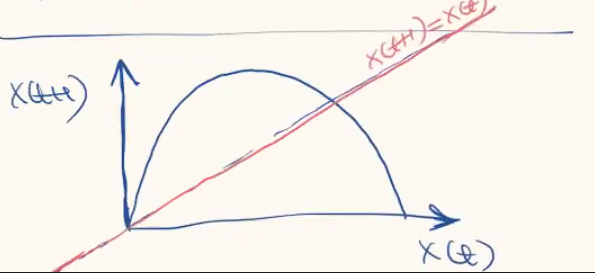
\includegraphics[width=250px]{C:/Users/Alex/Desktop/Notes/Spring 2021/pics/growth.png}
\end{example}

\textbf{TAG:} ModelingEvolution

\begin{remark}
	Why do we care about a basic model with wrong assumptions? Provides a basis for which we can compare parameters against(for example then varying popluation size and looking at divergence of effects from model).
\end{remark}

\begin{theme}
	Model cost(information cost to store) vs. model explanatory power. Some kind of ratio is the efficiency? Also how do we take into account the computational power necessary to answer questions.

	Applying computational complexity to model theory? Often computational complexity is applied to a single question. But maybe it should be applied to a theory answering a collection of questions? Allows for ammortized analysis of collection of questions.
\end{theme}

\begin{remark}
	How to model? Hard to say except use common sense. very complex. Important to understand what features we want to capture and make sure our model reflects parameters that take this into account.
\end{remark}


\end{document}

